\chapter{Diskuse a výsledky}

\section{Ověření funkčnosti systému}
Tato kapitola demonstruje praktickou funkčnost implementovaného systému na konkrétním příkladu hypotetického projektu venkovního posezení. Město plánuje instalaci stolu s~integrovanými lavicemi na místním sídlišti a~před realizací chce zjistit názor občanů. Správce proto vytvoří digitální dvojče tohoto posezení, které si mohou obyvatelé prohlédnout v~rozšířené realitě a~vyjádřit svůj názor. Následující sekce ukazují proces správy digitálního dvojčete správcem a~interakci koncového uživatele s~mobilní aplikací, čímž ověřují, že systém splňuje navržené požadavky.

\subsection{Správa digitálních dvojčat}
Správce zahajuje proces přidání nového projektu otevřením webové aplikace. Hlavní stránka webového rozhraní zobrazuje přehled projektů ve formě karet obsahujících náhledový obrázek, název, popis, souřadnice, průměrné hodnocení a~tlačítka pro správu, viz obrázek \ref{fig:web}.

\begin{figure}[H]
    \centering
    \includegraphics[width=\textwidth]{images/web_overview.png}
    \caption{Webové rozhraní s~přehledem projektů}
    \label{fig:web}
\end{figure}
\pagebreak
Správce klikne na tlačítko pro přidání projektu, které otevře modální formulář. Zde vyplňuje metadata projektu vyplní pole název, do popisu uvádí informace o~plánované instalaci venkovního posezení, doplňuje souřadnice lokality na sídlišti a~nahrává soubory (GLB model stolu s~lavicemi a~náhledový obrázek), viz obrázek \ref{fig:web_add}.

\begin{figure}[H]
    \centering
    \includegraphics[width=0.5\textwidth]{images/app_test_add.png}
    \caption{Formulář pro přidání nového projektu}
    \label{fig:web_add}
\end{figure}
V~případě potřeby má správce možnost projekt zcela odstranit. Smazání vyžaduje potvrzení a~odstraní projekt včetně všech přidružených souborů a~hodnocení, viz obrázek \ref{fig:web_delete}.

\begin{figure}[H]
    \centering
    \includegraphics[width=0.5\textwidth]{images/app_test_delete.png}
    \caption{Potvrzovací okno pro smazání}
    \label{fig:web_delete}
\end{figure}

Správce může také data následně upravit pomocí editačního formuláře. Pokud by například zadal špatné souřadnice nebo chtěl změnit popis projektu, může pomocí tohoto formuláře údaje opravit. Formulář je předvyplněn aktuálními daty a~umožňuje úpravu všech metadat i~nahrazení souborů, viz obrázek \ref{fig:web_edit}.
\begin{figure}[H]
    \centering
    \includegraphics[width=0.5\textwidth]{images/app_test_edit.png}
    \caption{Formulář pro úpravu existujícího projektu}
    \label{fig:web_edit}
\end{figure}


Po zveřejnění projektu s~posezením může veřejnost odesílat svou zpětnou vazbu. Správce má k~dispozici funkci pro zobrazení všech hodnocení projektu, kde vidí veškerou zpětnou vazbu. Hodnocení jsou seřazena chronologicky od nejnovějšího a~obsahují počet hvězdiček, volitelný komentář a~časové razítko. Tato zpětná vazba slouží městu k~vyhodnocení, zda obyvatelé sídliště instalaci posezení vítají, viz obrázek \ref{fig:web_rating}.

\begin{figure}[H]
    \centering
    \includegraphics[width=0.5\textwidth]{images/app_test_rating.png}
    \caption{Zobrazení hodnocení a~komentářů projektu}
    \label{fig:web_rating}
\end{figure}

\subsection{Interakce uživatele s~digitálními dvojčaty}
Obyvatel sídliště si chce prohlédnout plánované posezení a~vyjádřit svůj názor. Otevře mobilní aplikaci, která automaticky načte všechny dostupné projekty z~databáze. Aplikace zobrazí interaktivní mapové rozhraní s~vyznačenými pozicemi všech digitálních dvojčat, včetně bodu označujícího plánovanou lokaci posezení na sídlišti. Navigace v~mapě je intuitivní, uživatel ovládá zobrazení pomocí tlačítek pro přiblížení (+/-) a~čtyřsměrného ovladače pro posouvání. Aplikace dynamicky načítá nové mapové dlaždice při každé změně zobrazení a~průběžně přepočítává pozice bodů tak, aby odpovídaly aktuální mapové dlaždici.

Uživatel klikne na bod označující projekt s~posezením, čímž se otevře náhledový panel. Panel obsahuje název projektu, náhledový obrázek modelu, popis plánované instalace a~tlačítko pro zahájení vizualizace.

Po stisknutí tlačítka pro zahájení vizualizace aplikace plynule přejde do režimu rozšířené reality. Během tohoto přechodu se na pozadí stahuje 3D model stolu s~lavicemi ve formátu GLB. Jakmile je stahování dokončeno, model se automaticky zobrazí ve fyzickém prostředí uživatele, v~tomto případě přibližně ve vzdálenosti jednoho metru před ním. Toto umožňuje uživateli získat realistickou představu o~velikosti posezení a~posoudit, jak by mohlo vypadat v~reálném prostředí. V~AR režimu uživatel interaguje s~modelem prostřednictvím přirozených pohybů zařízení, může se volně pohybovat kolem objektu, přibližovat se pro detailnější prohlídku nebo se vzdalovat pro komplexnější pohled.

Po prohlédnutí modelu posezení může uživatel vyjádřit svůj názor prostřednictvím hodnotícího formuláře dostupného ze spodního navigačního panelu. Uživatel uděluje hodnocení pomocí hvězdiček v~rozsahu 1–5 a~může přidat volitelný textový komentář, například zda se mu samotný projekt líbí nebo zda má nějaké připomínky. Po odeslání systém validuje zadaná data a~ukládá je do databáze společně s~časovým razítkem, čímž umožňuje městu sledovat zpětnou vazbu obyvatel v~čase.

Uživatel se může vrátit na mapové rozhraní prostřednictvím navigačního panelu, kde může vybrat další projekt a~celý proces se opakuje.

\begin{figure}[H]
    \centering
    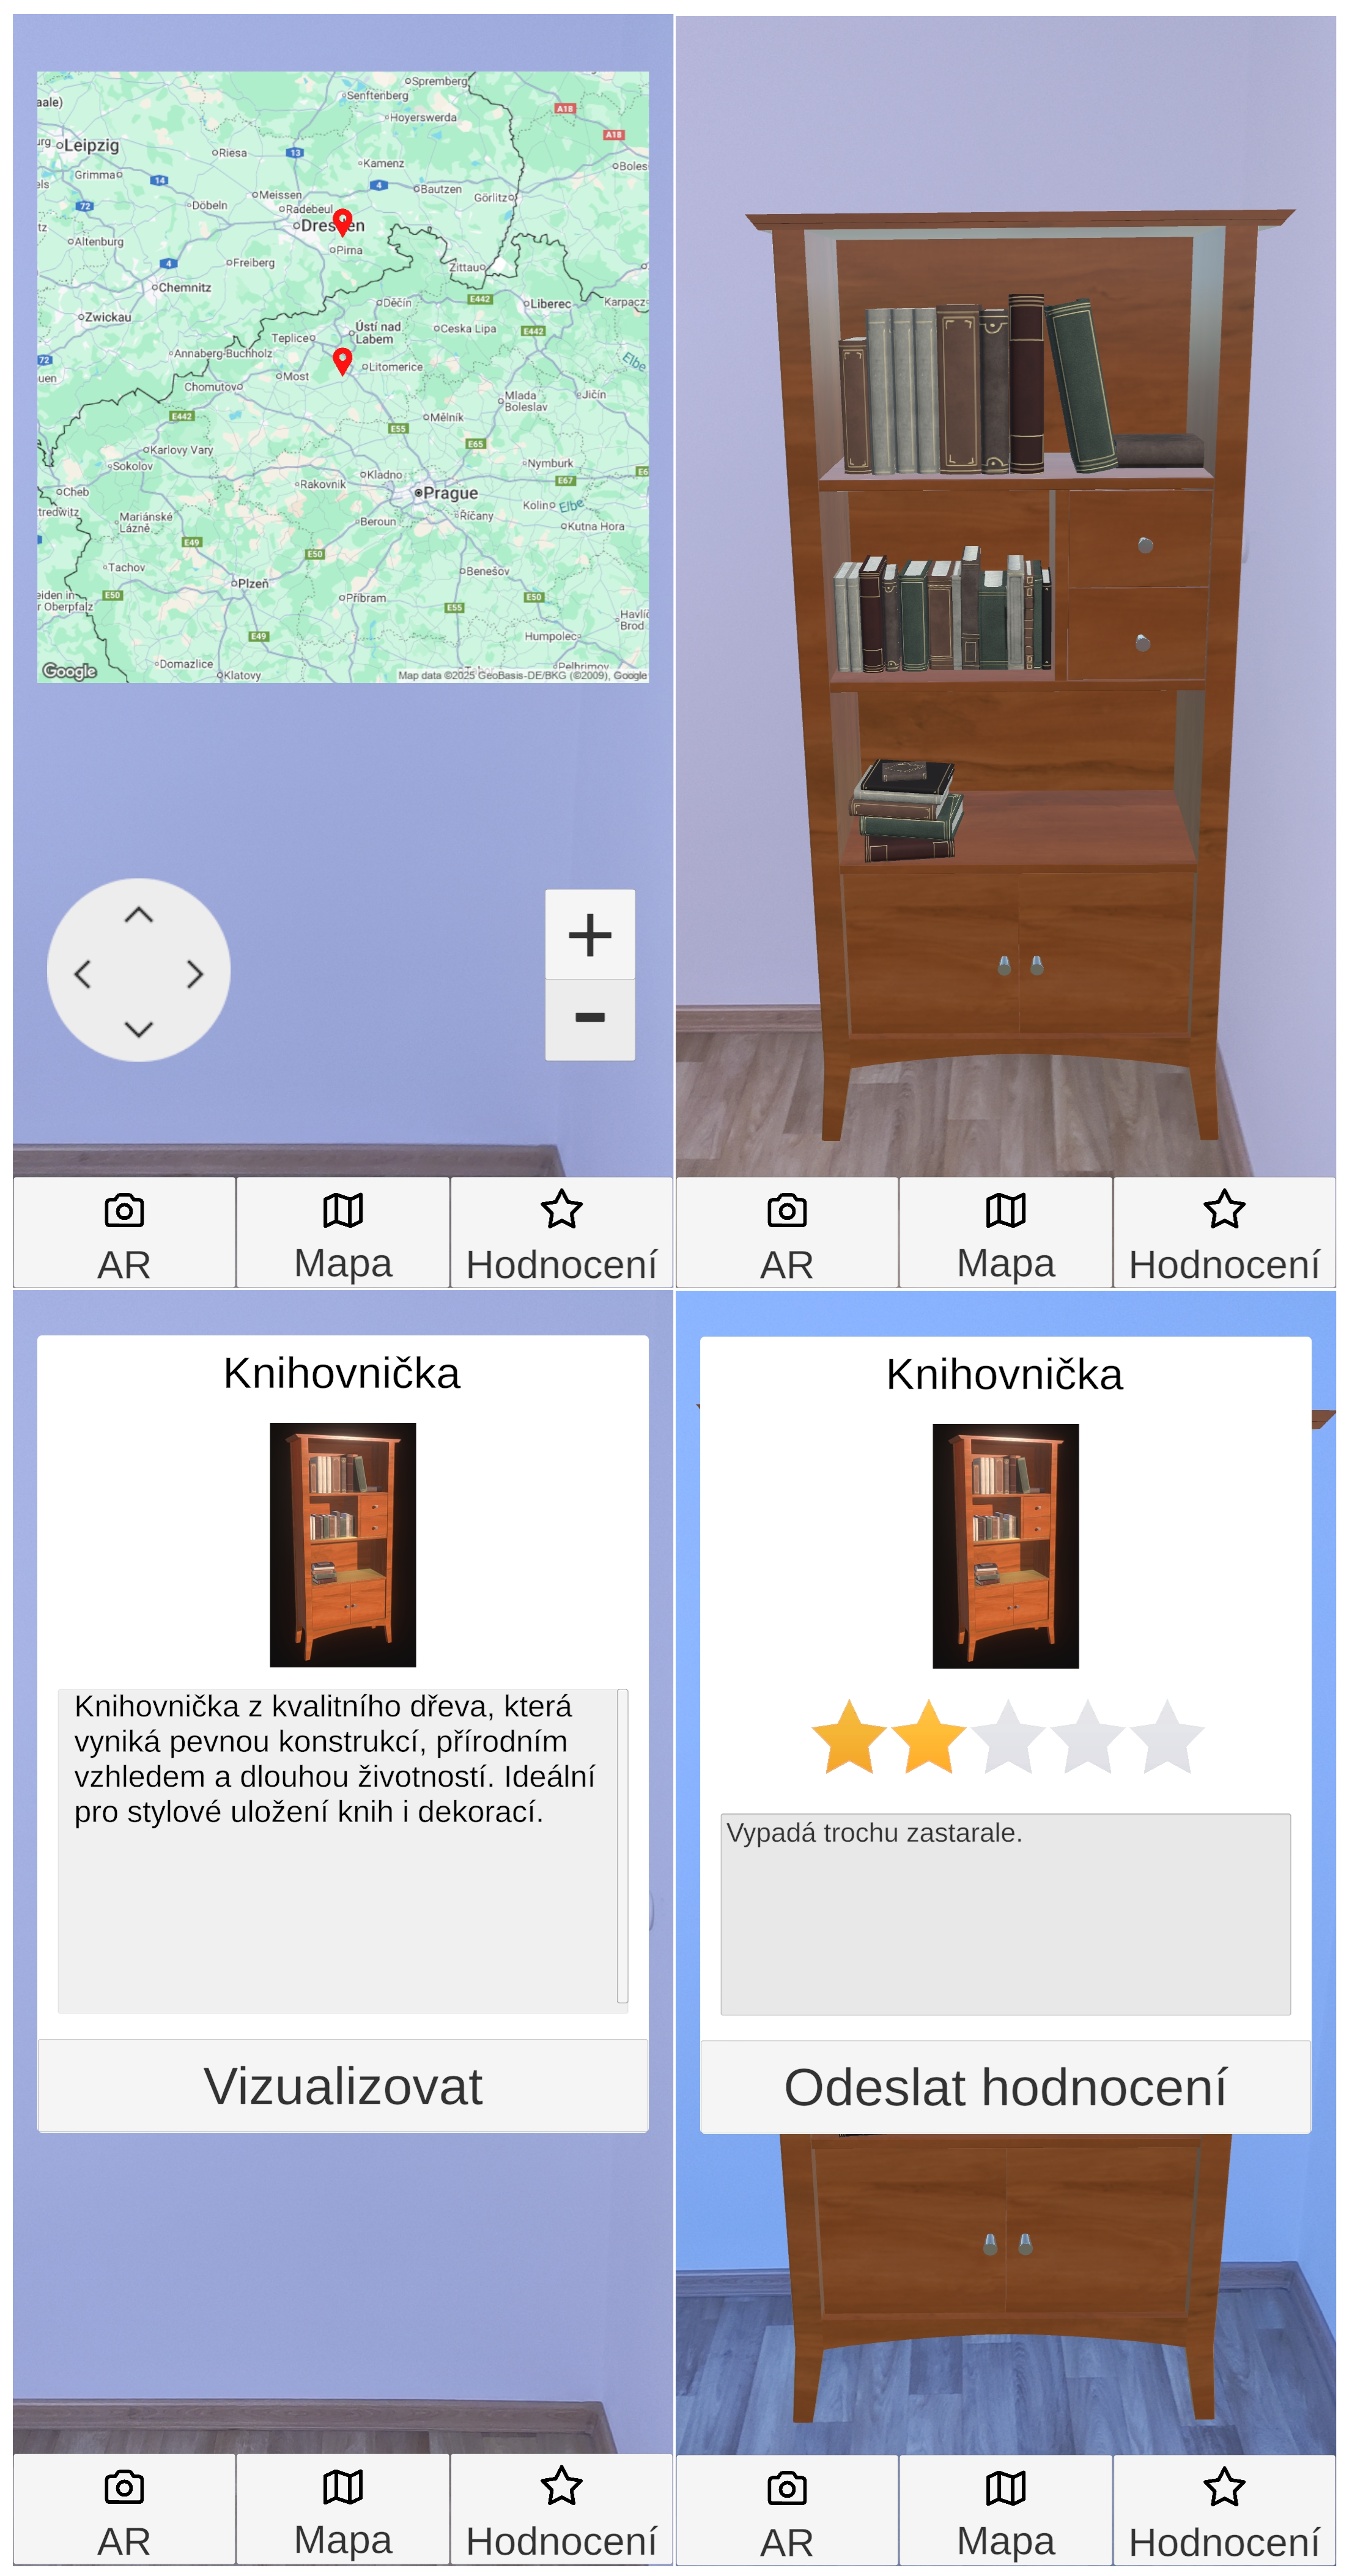
\includegraphics[width=0.77\textwidth]{images/mobile-app-showcase.png}
    \caption{Ukázka jednotlivých obrazovek v~mobilní aplikaci}
    \label{fig:map}
\end{figure}
\section{Hodnocení splnění cílů}

Hlavním cílem bylo vytvořit funkční prototyp pro zobrazení digitálních dvojčat v~rozšířené realitě.

Mobilní aplikace umožňuje zobrazení 3D modelů v~AR bez fyzických markerů, mapové rozhraní pro výběr projektů a zpětnou vazbu formou hodnocení a komentářů. Uživatelské rozhraní je intuitivní a aplikace je kompatibilní s Androidem.

Serverová část zajišťuje komunikaci přes REST API, správu digitálních dvojčat a implementuje cache mechanismus pro mapové dlaždice, což optimalizuje výkon a snižuje náklady na volání Google Maps API.

Webové rozhraní umožňuje správu projektů včetně nahrávání modelů, úprav a mazání. Webové rozhraní obsahuje také přehled všech projektů, který obsahuje všechny důležité údaje včetně zpětné vazby.

Během vývoje byly upraveny některé požadavky. Ukládání do osobního repozitáře bylo nahrazeno přímým načítáním ze serveru, což eliminuje zastaralá data a zjednodušuje architekturu. Skenování QR kódů nebylo implementováno, protože mapa opouští od nutnosti vylepovat QR kódy na reálná místa projektů. Detailní projektové informace (termíny, náklady, odpovědné firmy) nebyly zahrnuty, prototyp obsahuje obecný popis, který tyto informace může zahrnovat. V případě potřeby je datový model připraven na rozšíření. Otáčení modelu gestem nebylo implementováno, uživatel model prohlíží pohybem zařízení, což odpovídá přirozenému používání AR.
